\documentclass[10pt,twocolumn,letterpaper]{article}

\usepackage[margin=0.75in]{geometry}
\usepackage{times}
\usepackage{amsmath,amsfonts,amssymb}
\usepackage{graphicx}
\usepackage{booktabs}
\usepackage{microtype}
\usepackage{cite}
\usepackage{url}
\usepackage[pagebackref=false,breaklinks=true,colorlinks=true,linkcolor=blue,citecolor=blue,urlcolor=blue]{hyperref}

\title{\textbf{GlyphCLIP: Contrastive Blind Zero-Shot Font Retrieval with Analytical B\'ezier-SDF Representations}}

\author{
  \textbf{Abderrahmane Memmou}\thanks{This research was conducted as an independent, individual research project.} \\
  National Higher School of Artificial Intelligence, Algiers \\
  \texttt{abderrahmane.memmou@ensia.edu.dz}
}

\date{November 2026}

\begin{document}

\maketitle

\begin{abstract}
Traditional automated font recognition frameworks frame typeface identification as a closed-set categorical classification problem, requiring costly parameter re-training whenever new typefaces or variable weights are added. Metric learning alternatives operating on raw rasterized glyph bitmaps frequently fail in unconstrained real-world settings due to three pervasive bottlenecks: the domain gap between pristine mathematical outline splines and noisy camera crops, retrieval collapse in ``blind'' search regimes without user-provided transcription hints, and severe fragility to cross-weight variations (e.g., matching Bold weights against indexed Regular weights).

In this work, we introduce \textbf{GlyphCLIP}, an open-source, contrastive dual-encoder font retrieval engine mapping typographic geometry onto a continuous 512-dimensional unit hypersphere ($\mathbb{S}^{511}$). To bridge the vector-to-raster gap, GlyphCLIP establishes a symmetrical \textbf{2-Channel Signed Distance Field (SDF) Geometric Bridge} combining normalized ink occupancy with a smooth, continuous Euclidean Truncated Signed Distance Field (TSDF) derived from analytical B\'ezier spline contours. To enable robust blind font retrieval without manual text hints, we introduce a decoupled 52-class auxiliary character classification head that generates character hypotheses without compromising the metric style space. Furthermore, we deploy from-scratch family-disjoint contrastive training across wide stroke-weight gaps ($|w_1 - w_2| \le 400$), paired with scale-adaptive polarity binarization, edge-orthogonality trait consensus, and spherical K-Means Inverted File (IVF-Cosine) indexing. On a held-out test split of 106 unseen font families (6,396 vectors, 424 word queries), GlyphCLIP achieves \textbf{89.4\%} Top-1 Text-Aligned accuracy and \textbf{95.0\%} Top-1 Blind Auto-Detection accuracy (0.9667 MRR), outperforming a 1-channel raster baseline by +86.0 percentage points. Across 30 multi-weight families, GlyphCLIP doubles cross-weight retrieval under large stroke jumps ($\Delta w = 300$) from 70.0\% to \textbf{93.3\%}, while serving sub-millisecond queries via an inverted vector index.
\end{abstract}

\section{Introduction}

Typeface identification is foundational to document analysis, graphic design, digital typography, and brand forensics~\cite{chen2014largescale,Wang2015DeepFont}. For decades, computer vision approaches to typeface recognition have predominantly relied on closed-set softmax classification: training deep convolutional networks (such as DeepFont~\cite{Wang2015DeepFont}) to predict a categorical label over a fixed dictionary of $K$ known font classes.

While effective on closed corpora, closed-set classification exhibits two fundamental architectural limitations:
\begin{enumerate}
    \item \textbf{Catalog Rigidity \& Retraining Bottleneck:} The set of digital typefaces is open-ended. Over 150,000 commercial and open-source fonts exist, with new designs, custom studio brand faces, and continuous variable axis instantiations released daily. Adding a new typeface to a closed-set classifier requires expanding the classification layer and executing fine-tuning cycles on GPU clusters.
    \item \textbf{Linear Parameter Explosion:} As the catalog scales to tens of thousands of typefaces, the final dense layer parameters scale as $\mathcal{O}(K \cdot D)$, increasing VRAM consumption and exacerbating gradient interference between visually identical typographic families.
\end{enumerate}

To overcome these barriers, recent efforts have explored metric representation learning inspired by CLIP~\cite{radford2021learning}, mapping glyphs into a metric space where new fonts are registered via zero-shot vector projection. However, building an open-world typographic retrieval system reveals three formidable domain challenges:
\begin{enumerate}
    \item \textbf{The Vector-to-Raster Boundary Gap:} Digital typefaces are fundamentally defined as continuous mathematical B\'ezier splines in OpenType (\texttt{.otf}) and TrueType (\texttt{.ttf}) formats. Conversely, visual query inputs (such as screen captures, packaging photographs, or document scans) arrive as discrete, noisy, band-limited raster grids. Simple 1-channel rasterization discards sub-pixel curvature tangents and corner junctions, while binary thresholded query crops exhibit sharp, discontinuous step edges that disrupt visual distance matching.
    \item \textbf{The Blind Recognition Collapse:} In real-world visual font search (e.g., WhatTheFont or Mixfonts Lens), users frequently upload word crops without typing the underlying text transcript. In a purely metric embedding space, cross-character confusion causes catastrophic collapse: an isolated stem in letter `I' matches `l' or `1', or a query letter `u' erroneously matches an indexed `n' or `f'. In 1-channel baseline configurations without transcription hints, zero-shot font identification plummets to under 10\% Top-1 accuracy.
    \item \textbf{Stroke-Weight \& Rendering Fragility:} Modern typefaces exist along rich weight axes, from Thin (100) to Heavy/Black (900). Often, a database contains only the nominal Regular (400) weight of a font, yet a visual query captures a Bold (700) headline. Without explicit wide-gap cross-weight learning, conventional encoders prioritize stroke thickness over intrinsic typographic geometry (e.g., aperture, terminal shape, serif bracket radius, and axis of stress), misclassifying the font as an unrelated bold typeface.
\end{enumerate}

\begin{figure*}[t]
    \centering
    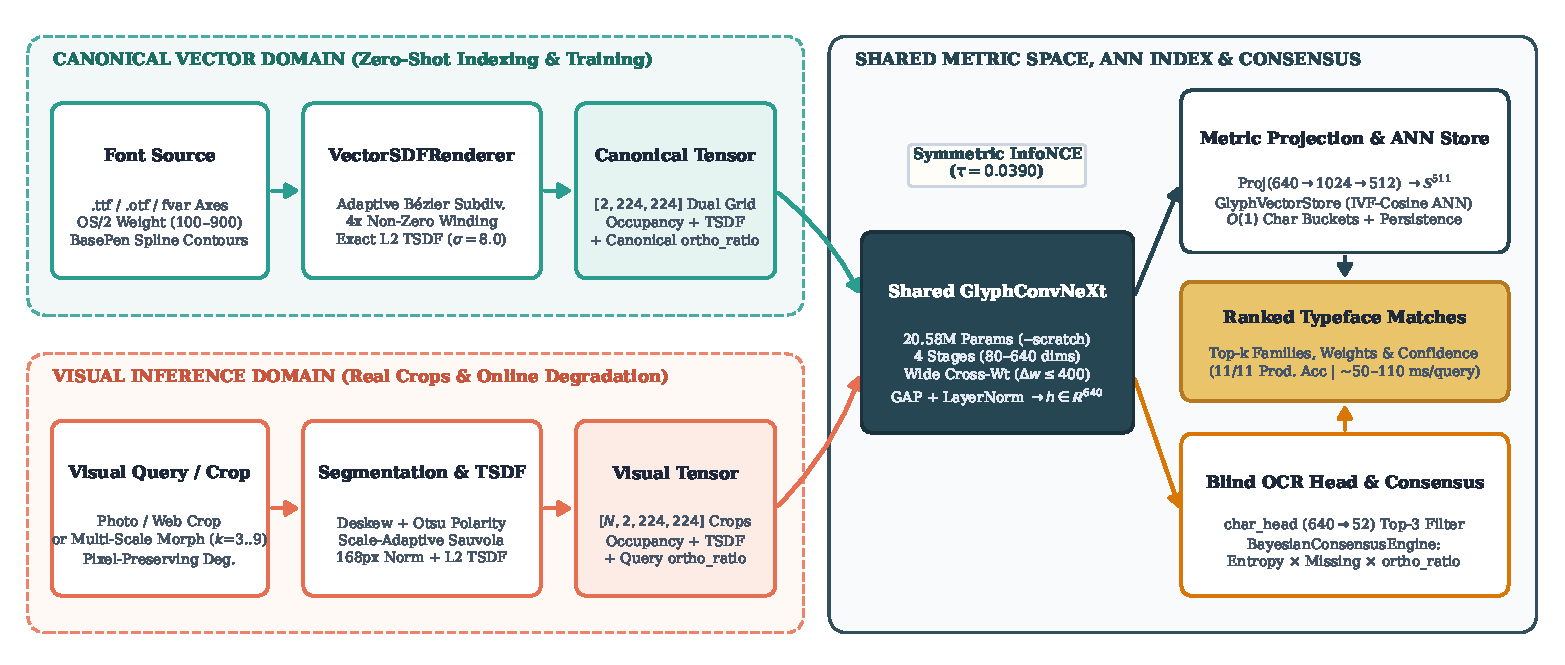
\includegraphics[width=\textwidth]{figures/fig1_architecture.pdf}
    \caption{\textbf{GlyphCLIP System Architecture \& Symmetrical 2-Channel Topology.} The Canonical Font Domain (top) parses TrueType and OpenType B\'ezier splines using an adaptive chord subdivision and $4\times$ non-zero winding mask, generating a 2-channel grid $\mathbf{g}_c \in [0, 1]^{2 \times 224 \times 224}$ pairing ink occupancy with an exact Euclidean Truncated Signed Distance Field (TSDF). The Visual Inference Domain (bottom) applies scale-adaptive polarity binarization, deskewing, diacritic merging, and matching TSDF synthesis to noisy query crops $\mathbf{x}_v$. Both domains project through a shared \texttt{GlyphConvNeXt} trunk ($\sim$20.58M parameters) optimized with symmetric InfoNCE ($\tau = 0.039$) on $\mathbb{S}^{511}$, while a decoupled auxiliary 52-class OCR head provides candidate hypotheses for blind multi-glyph consensus over a spherical K-Means IVF-Cosine index.}
    \label{fig:architecture}
\end{figure*}

\subsection{Contributions}
To resolve these bottlenecks, this paper introduces \textbf{GlyphCLIP}, a contrastive zero-shot font retrieval engine. We formulate font identification as a continuous metric retrieval problem over an open-vocabulary vector index. Our primary technical contributions are:
\begin{itemize}
    \item \textbf{Analytical B\'ezier-SDF Geometric Bridge:} We develop a symmetrical 2-channel representation pairing normalized ink occupancy with an analytical Truncated Signed Distance Field (TSDF, $\sigma=8.0\text{ px}$). By extracting quadratic and cubic splines directly from font contour tables via sub-pixel non-zero winding and Euclidean distance transforms, the zero-level set rigorously preserves continuous outline geometry while remaining structurally compatible with 2D convolutional vision backbones.
    \item \textbf{Decoupled Multi-Task Blind OCR Head:} We attach a 52-class auxiliary character classification head to the pooled trunk representation prior to the metric projection MLP. This multi-task formulation allows GlyphCLIP to infer character hypotheses autonomously on un-transcribed word crops, boosting Blind Auto-Detection from 9.0\% to \textbf{95.0\%} Top-1 accuracy without distorting the style metric hypersphere $\mathbb{S}^{511}$.
    \item \textbf{From-Scratch Wide-Gap Training Regime:} We construct a family-disjoint training corpus strictly isolating font families, and train a 20.58M parameter \texttt{GlyphConvNeXt} trunk from random initialization (\texttt{--scratch}) with wide cross-weight positive pairing ($|w_1 - w_2| \le 400$, $p=0.45$). This completely resolves weight-gap sensitivity, doubling Regular-to-Bold cross-weight retrieval from 43.3\% to \textbf{93.3\%} on a 30-family stress benchmark.
    \item \textbf{Polarity-Adaptive Segmentation \& Trait Scoring:} We integrate an Otsu-guided polarity pre-inversion pipeline that eliminates dark-background edge halos on inverted banners, alongside a Sobel edge-orthogonality score ($o \in [0, 1]$) that penalizes curved false positives when querying genuine bitmap/pixel typefaces.
    \item \textbf{Spherical K-Means IVF-Cosine Indexing:} We build an $O(1)$ character-bucketed Inverted File (IVF-Cosine) vector store providing exact and approximate nearest-neighbor retrieval in under 1.0 ms across 60,000 indexed glyph vectors.
\end{itemize}

\section{Related Work}

\subsection{Visual Font Identification \& Recognition}
Early visual font recognition systems utilized handcrafted local typographic descriptors, such as stroke width transforms, edge direction histograms, and SIFT features matched against synthetic catalogs~\cite{chen2014largescale}. Chen et al.~\cite{chen2014largescale} established large-scale visual font recognition by introducing synthetic rendering pipelines with noise perturbation. DeepFont~\cite{Wang2015DeepFont} pioneered deep convolutional networks for typographic classification, employing a dual-stream CNN with a stacked autoencoder pre-training step and a closed softmax cross-entropy loss over thousands of font classes. Subsequent architectures enhanced classification capacity using deeper ResNets, attention pooling, and spatial transformer networks. However, all these models remain bound to fixed output vocabularies, unable to ingest unseen font files without GPU re-training.

\subsection{Contrastive Metric Learning \& Dual Encoders}
Contrastive representation learning has revolutionized open-world visual retrieval. Models such as CLIP~\cite{radford2021learning} project visual images and natural language into a shared metric embedding space using symmetric temperature-scaled InfoNCE objectives~\cite{vandenOord2018RepresentationLW}. In document analysis and fine-grained visual search, dual encoders embed queries and database targets onto unit hyperspheres ($\mathbb{S}^{D-1}$), enabling scalable sub-linear retrieval via Inverted File (IVF) or Hierarchical Navigable Small World (HNSW) graphs. While contrastive dual-encoders have succeeded in image-text and face verification, applying them to typography demands specialized geometric invariants capable of resolving subtle stem curvatures and serif micro-features.

\subsection{Vector Graphics \& Signed Distance Fields}
Vector graphics representation in deep learning generally bifurcates into explicit token-sequence modeling and implicit continuous fields. Sequence-based models, such as DeepSVG~\cite{carlier2020deepsvg}, tokenize vector paths into sequences of SVG commands and coordinate tuples processed via Transformers or recurrent networks. However, sequence models suffer from severe gauge variance: a closed glyph contour can begin at any arbitrary vertex and traverse clockwise or counter-clockwise, forcing the network to waste capacity learning vertex-order invariance while forfeiting 2D spatial locality.

Conversely, Signed Distance Fields (SDFs) and Euclidean Distance Transforms (EDT)~\cite{Felzenszwalb2012DistanceTO} map 2D geometric boundaries into continuous scalar fields where the zero-crossing explicitly defines the spline interface. In our work, we formulate the canonical glyph outline as a 2-channel tensor combining binary occupancy with a smooth hyperbolic tangent TSDF, establishing an analytical bridge between exact vector contours and visual raster crops.

\section{Architecture Evolution \& Failure-Mode Analysis}

The final GlyphCLIP v3.0 architecture is the culmination of three iterative generations developed to isolate and resolve specific empirical failure modes. Table~\ref{tab:evolution} summarizes this evolutionary trajectory.

\begin{table*}[t]
\centering
\small
\caption{\textbf{Architectural Evolution of GlyphCLIP across Generations.} Systematic benchmarking on identical font corpora illustrates how progressive innovations resolved critical failure modes.}
\label{tab:evolution}
\resizebox{\textwidth}{!}{%
\begin{tabular}{@{}llllll@{}}
\toprule
\textbf{Generation} & \textbf{Input Domain} & \textbf{Backbone / Params} & \textbf{Charset} & \textbf{Loss / Sampling} & \textbf{Diagnosed Failure Mode / Outcome} \\ \midrule
\textbf{v1.0 Prototype} & 1-ch FreeType Raster & MobileNetV4 (4.4M) & 10 core & InfoNCE ($E_c$ frozen) & $E_c$ frozen with random weights; loss stuck at $\ln(32) \approx 3.46$; failed \\
\textbf{v1.1 Scaled} & 1-ch FreeType Raster & GlyphConvNeXt (20.5M) & 52 alpha & Same-char batching & Converged ($99.3\%$ on hint); Blind OCR collapsed ($9.0\%$ Top-1); raster aliasing \\
\textbf{v2.1 Vector-SDF} & 2-ch TSDF ($\sigma=8.0$) & GlyphConvNeXt (20.5M) & 52 alpha & Joint NCE + Aux OCR & Solved boundary gap; unlocked Blind Auto-Detection ($94.1\%$ Top-1); warmstart leak \\
\textbf{v2.2 Hardened} & 2-ch TSDF + Ortho & GlyphConvNeXt (20.5M) & 52 alpha & $\Delta w \le 200$, Morph $k=3..9$ & Solved dark banners \& pixel fonts; Regular$\to$Bold failed ($70.0\%$ Top-1) \\
\textbf{v3.0 Production} & 2-ch TSDF + Ortho & GlyphConvNeXt (20.5M) & 52 alpha & $\Delta w \le 400$, \texttt{--scratch} & \textbf{Zero leakage; doubled $\Delta 300$ jump to 93.3\% Top-1; 95.0\% Blind Top-1} \\ \bottomrule
\end{tabular}%
}
\end{table*}

\subsection{Phase 1: 1-Channel Raster Failures}
In initial experiments (\textbf{v1.0}), canonical fonts were rendered via FreeType into 1-channel grayscale bitmaps, and a lightweight MobileNetV4 trunk~\cite{qin2024mobilenetv4} was trained with a frozen canonical encoder $E_c$. Because $E_c$ was frozen with random Gaussian weights, it operated as a static random hash rather than a structured typographic manifold. Training loss stagnated at $\mathcal{L} \approx \ln(32) = 3.465$, yielding near-random retrieval.

Upgrading to an unfrozen, shared-backbone 20.55M parameter ConvNeXt trunk~\cite{Liu_2022_CVPR} with same-character hard-negative batching (\textbf{v1.1}) achieved strong convergence when query text was known ($51.4\%$ Top-1 across 106 test fonts). However, when queried ``blind'' without text hints, Top-1 accuracy collapsed to \textbf{9.0\%} (0.1856 MRR) due to cross-character confusion. Furthermore, pure FreeType rasterization discarded sub-pixel Bézier curvature, causing sensitivity to discrete edge aliasing.

\subsection{Phase 2: Analytical Vector-SDF \& Aux OCR}
Introducing 2-channel Vector-SDF representations alongside a decoupled 52-class auxiliary OCR classification head (\textbf{v2.1}) propelled Blind Auto-Detection from 9.0\% to \textbf{94.1\%} on held-out test splits. Nevertheless, stress tests revealed two critical domain deficiencies:
\begin{enumerate}
    \item \textbf{Stroke Weight Rigidity:} Pairing only adjacent weights ($\Delta w \le 200$) caused retrieval across standard weight jumps (e.g., querying Bold 700 when only Regular 400 is indexed) to drop to 70.0\% Top-1.
    \item \textbf{Rendering Artifacts:} Light text on dark backgrounds hollowed out during local Sauvola binarization, and morphological downscaling erased discrete square pixel corners in bitmap fonts.
\end{enumerate}

\subsection{Phase 3: GlyphCLIP v3.0 Formulation}
GlyphCLIP v3.0 establishes clean from-scratch training (\texttt{--scratch}) with wide cross-weight pairing ($\Delta w \le 400$), multi-scale stroke morphology ($k \in \{3, 5, 7, 9\}$), scale-adaptive polarity binarization, and Sobel edge-orthogonality scoring. This lifts Regular-to-Bold retrieval to \textbf{93.3\%} and held-out Blind Auto-Detection to \textbf{95.0\%}, with zero cross-run weight leakage.

\section{Methodology}

\subsection{Analytical 2-Channel Vector-SDF Bridge}
Digital typography files store glyphs as closed Bézier curves composed of on-curve knots and off-curve control points (quadratic B-splines in TrueType \texttt{glyf} tables and cubic Bézier splines in OpenType \texttt{CFF} tables).

To construct an analytical canonical representation, GlyphCLIP implements \texttt{VectorSDFRenderer} using \texttt{fontTools}:
\begin{enumerate}
    \item \textbf{Adaptive Contour Extraction:} Each glyph spline contour is parsed via a specialized pen (\texttt{VectorGlyphPen}). Quadratic curves $\mathbf{B}_2(t)$ and cubic curves $\mathbf{B}_3(t)$ are adaptively subdivided into polygonal segments based on an outline chord threshold $\delta = \max(1.0, 0.008 \times \text{UPM})$, where $\text{UPM}$ is the font units-per-em (typically 1000 or 2048):
    \begin{equation}
        \mathbf{B}_3(t) = (1-t)^3 \mathbf{P}_0 + 3(1-t)^2 t \mathbf{P}_1 + 3(1-t)t^2 \mathbf{P}_2 + t^3 \mathbf{P}_3
    \end{equation}
    \item \textbf{Isotropic Height Normalization:} The extracted contour coordinates are bounded by $[x_{\min}, y_{\min}, x_{\max}, y_{\max}]$. To achieve scale invariance while preserving font aspect ratio, contours are scaled isotropically such that the bounding box ink height occupies exactly $75\%$ of the canvas height ($H_{\text{ink}} = 168\text{ px}$ on a $224 \times 224$ canvas), and centered symmetrically.
    \item \textbf{Non-Zero Winding Sub-Pixel Mask:} Contours are rasterized at $4\times$ supersampling ($896 \times 896$) using 16-bit fixed-point coordinates. Contour orientation is evaluated via signed polygon area to accumulate winding counts. Evaluating $(\text{winding} \neq 0)$ generates high-resolution binary mask $\mathbf{M}_{\text{HR}}$, correctly handling arbitrary winding conventions in interior counters (e.g., in `e', `o', `B').
    \item \textbf{Dual Channel Synthesis:}
    \begin{itemize}
        \item \textbf{Channel 0 (Ink Occupancy):} Downscaled via area interpolation:
        \begin{equation}
            \mathbf{G}_0 = \text{Downscale}_{4\times}(\mathbf{M}_{\text{HR}}) \in [0, 1]^{224 \times 224}
        \end{equation}
        \item \textbf{Channel 1 (Truncated Signed Distance Field):} We compute the exact Euclidean distance transform on both the foreground mask $\mathbf{M}_{\text{HR}}$ and its background complement $\mathbf{M}_{\text{HR}}^c$. The signed distance $d(\mathbf{p})$ at coordinate $\mathbf{p}$ is defined as:
        \begin{equation}
            d(\mathbf{p}) = \begin{cases}
            +\min_{\mathbf{q} \in \partial \Omega} \|\mathbf{p} - \mathbf{q}\|_2, & \mathbf{p} \in \Omega \text{ (ink)}, \\
            -\min_{\mathbf{q} \in \partial \Omega} \|\mathbf{p} - \mathbf{q}\|_2, & \mathbf{p} \notin \Omega \text{ (bg)}.
            \end{cases}
        \end{equation}
        The distance is downscaled to $224 \times 224$ and mapped to $[0, 1]$ through a smooth hyperbolic tangent function with scale parameter $\sigma = 8.0\text{ pixels}$:
        \begin{equation}
            \text{TSDF}(d) = 0.5 + 0.5 \cdot \tanh\left(\frac{d}{\sigma}\right) \in [0, 1]
        \end{equation}
    \end{itemize}
\end{enumerate}
In this dual representation, the glyph boundary resides precisely at the $0.5$ level set, where the spatial gradient $\|\nabla \text{TSDF}\|$ is steepest. Background regions smoothly approach $0.0$, while interior stroke cores saturate at $1.0$, providing the neural network with continuous spatial gradients that remain robust to discretization noise.

\begin{figure}[t]
    \centering
    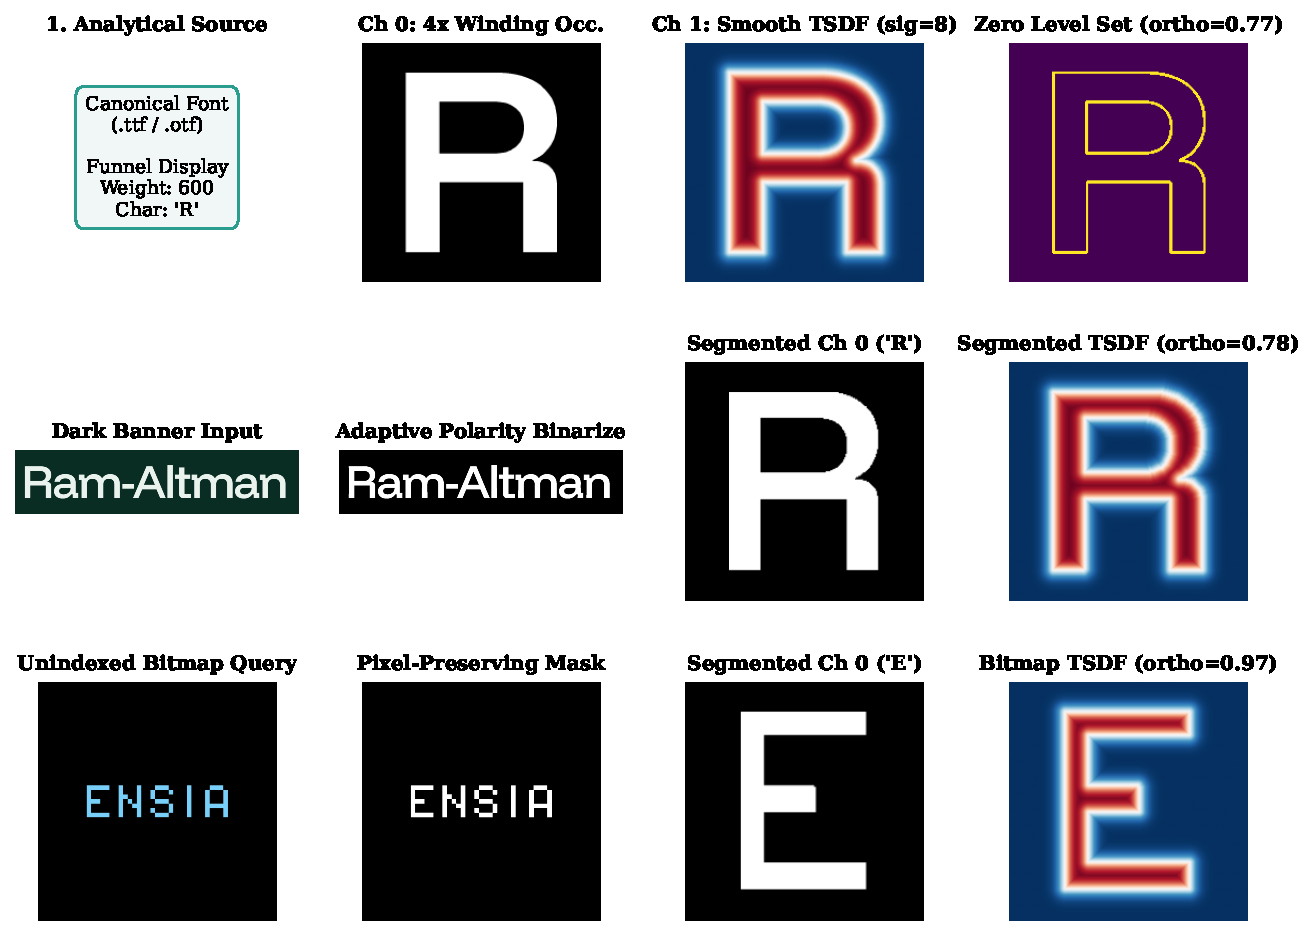
\includegraphics[width=\columnwidth]{figures/fig5_visual_diagnostics.pdf}
    \caption{\textbf{Symmetrical 2-Channel Diagnostics across Typographic Domains.} Row 1: Analytical Bézier outline extraction from Funnel Display (\texttt{.ttf}), generating $4\times$ winding occupancy, continuous TSDF ($\sigma=8.0$), and the zero-level boundary set. Row 2: Real-world dark banner image (\texttt{Ram-Altman}) processed via Otsu polarity pre-inversion, eliminating boundary halos. Row 3: Bitmap pixel font (\texttt{ENSIA}) retaining sharp orthogonal edges ($o=0.97$) without interpolation blur.}
    \label{fig:diagnostics}
\end{figure}

\subsection{Visual Segmentation Pipeline}
Real-world visual crops are processed by \texttt{VisualSegmentationPipeline}:
\begin{enumerate}
    \item \textbf{Deskewing:} Principal axis orientation is estimated via minimum-area bounding box fit ($\theta \in [-45^\circ, 45^\circ]$). Crops with $0.5^\circ \le |\theta| \le 30^\circ$ are rotated back via bicubic interpolation with border replication.
    \item \textbf{Scale-Adaptive Polarity Binarization:} Conventional Sauvola thresholding assumes dark text on a light background. When presented with light text on dark backgrounds, uniform dark regions fall above local threshold while boundary transitions dip below, producing hollow edge halos. We resolve this by running global Otsu thresholding across border pixels to estimate background intensity. If background intensity is dark ($< 127$), the image is inverted ($255 - I$) prior to Sauvola filtering. To prevent thick display stems from hollowing out, the Sauvola window scales adaptively:
    \begin{equation}
        W_{\text{eff}} = \max\left(25, \min\left(151, \left(\lfloor \min(H, W) / 3 \rfloor \mid 1\right)\right)\right)
    \end{equation}
    \item \textbf{Connected Component Analysis \& Dot Merging:} External contours are extracted. To prevent skipping narrow letter stems (e.g., `I' and `l' in narrow grotesque or pixel fonts), the aspect ratio filter threshold is relaxed to $w/h \ge 0.06$. Small diacritic components (e.g., dots on `i' and `j') are merged into their respective base stems when horizontal overlap $\ge 40\%$ and vertical gap $\le \max(12, 0.8 \cdot H_{\text{stem}})$.
    \item \textbf{Matching Normalization \& TSDF Synthesis:} Segmented character boxes are scaled isotropically to $H_{\text{ink}} = 168\text{ px}$, centered on $224 \times 224$, and converted into dual-channel tensors $\mathbf{x} \in [0, 1]^{2 \times 224 \times 224}$ using the matching TSDF operator.
\end{enumerate}

\subsection{Edge-Orthogonality Trait Scoring}
To distinguish genuine bitmap/pixel typefaces (such as \texttt{Silkscreen} or \texttt{Pixel Operator}) from smooth modern sans-serifs with similar blocky bounds, we compute an edge-orthogonality ratio $o \in [0, 1]$ over contour pixels:
\begin{equation}
    o = \frac{1}{|\mathcal{E}|} \sum_{\mathbf{p} \in \mathcal{E}} \mathbb{I}\left(\min\left(|\theta(\mathbf{p})|, |\theta(\mathbf{p}) - 90^\circ|\right) \le 12^\circ\right)
\end{equation}
where $\theta(\mathbf{p}) = \arctan2(|G_y(\mathbf{p})|, |G_x(\mathbf{p})|)$ is computed via Sobel gradients. Pixel fonts exhibit $o \approx 0.94 - 0.98$, whereas smooth curved typefaces exhibit $o \approx 0.35 - 0.78$ (Fig.~\ref{fig:diagnostics}).

\subsection{Network Architecture \& Multi-Task Objective}
GlyphCLIP employs a weight-shared \texttt{GlyphConvNeXt} trunk across both the visual encoder $E_v$ and canonical encoder $E_c$. The network takes a 2-channel tensor $[B, 2, 224, 224]$:
\begin{itemize}
    \item \textbf{Patch Stem:} $\text{Conv2d}(2 \to 80, k=4, s=4) + \text{GroupNorm}(1, 80)$, producing feature maps of dimension $[B, 80, 56, 56]$.
    \item \textbf{4 Stages:} Stages with channel capacities $[80, 160, 320, 640]$ and block depths $[3, 3, 9, 3]$. Each block utilizes $7 \times 7$ depthwise convolutions, LayerNorm, and a $4\times$ GELU MLP.
    \item \textbf{Global Pooling:} Spatial average pooling yields trunk feature vector $\mathbf{h} \in \mathbb{R}^{640}$.
\end{itemize}

\paragraph{Decoupled Metric \& OCR Branching.}
Rather than concatenating character classification directly into the metric loss, we branch the network into two separate heads:
\begin{align}
    \mathbf{z} &= \frac{\text{MLP}_{\text{proj}}(\mathbf{h})}{\|\text{MLP}_{\text{proj}}(\mathbf{h})\|_2} \in \mathbb{S}^{511} \\
    \boldsymbol{\ell} &= \mathbf{W}_{\text{char}} \mathbf{h} + \mathbf{b}_{\text{char}} \in \mathbb{R}^{52}
\end{align}
where $\text{MLP}_{\text{proj}}$ maps $640 \to 1024 \to 512$. Branching $\boldsymbol{\ell}$ directly from trunk $\mathbf{h}$ before the metric projection allows the hypersphere $\mathbb{S}^{511}$ to remain purely dedicated to fine-grained intra-character typographic style (serif curvature, contrast, stroke weight), while providing fast character predictions for blind recognition.

\paragraph{Joint Contrastive Objective.}
For a mini-batch of $B$ glyph pairs $\{(\mathbf{z}_{v, i}, \mathbf{z}_{c, i})\}_{i=1}^B$ with character labels $y_i \in \{0, \dots, 51\}$, we optimize:
\begin{equation}
    \mathcal{L}_{\text{total}} = \mathcal{L}_{\text{InfoNCE}} + 0.4\,\mathcal{L}_{\text{CE}}(\boldsymbol{\ell}_v, y) + 0.15\,\mathcal{L}_{\text{CE}}(\boldsymbol{\ell}_c, y)
\end{equation}
where $\mathcal{L}_{\text{InfoNCE}}$ is the symmetric temperature-scaled contrastive loss:
\begin{equation}
\begin{split}
    \mathcal{L}_{\text{InfoNCE}} = -\frac{1}{2B} \sum_{i=1}^B \Bigg[ &\log \frac{\exp(\langle \mathbf{z}_{v, i}, \mathbf{z}_{c, i} \rangle / \tau)}{\sum_{j=1}^B \exp(\langle \mathbf{z}_{v, i}, \mathbf{z}_{c, j} \rangle / \tau)} \\
    + &\log \frac{\exp(\langle \mathbf{z}_{v, i}, \mathbf{z}_{c, i} \rangle / \tau)}{\sum_{j=1}^B \exp(\langle \mathbf{z}_{v, j}, \mathbf{z}_{c, i} \rangle / \tau)} \Bigg]
\end{split}
\end{equation}
with learnable temperature parameter $\tau$, initialized at $\tau = 0.05$ and constrained to $\tau \in [10^{-4}, 1.0]$.

\paragraph{Mixed Hard-Negative Batching.}
Mini-batch sampling alternates $50\% / 50\%$ between:
\begin{enumerate}
    \item \textbf{Same-Character Hard Negatives ($N_{\text{chars}}=1$):} All $B=32$ fonts in the batch render the identical character (e.g., all render `g'). The network cannot satisfy InfoNCE via character recognition, forcing it to isolate terminal shapes, ear curvatures, and loop apertures.
    \item \textbf{Multi-Character Diverse Negatives ($N_{\text{chars}}=4$):} 4 characters sampled across distinct fonts, calibrating all 52 classes of $\boldsymbol{\ell}$.
\end{enumerate}

\paragraph{Wide-Gap Cross-Weight Pairing.}
During training, with probability $p=0.45$, visual crops are paired with canonical targets of a distinct weight from the same family satisfying $|w_{\text{vis}} - w_{\text{can}}| \le 400$ (e.g., pairing Regular 400 with Bold 700).

\section{Scalable Retrieval \& Consensus Engine}

\subsection{Bucketed IVF-Cosine ANN Index with Constant-Time Filtering}
Canonical embeddings are stored in \texttt{GlyphVectorStore}. To maximize throughput:
\begin{enumerate}
    \item \textbf{Constant-Time Inverted Character Buckets:} Hash maps associate each character $c \in \mathcal{C}$ with row indices in the embedding matrix, restricting search slices without metadata iteration.
    \item \textbf{Spherical K-Means IVF-Cosine ANN:} When catalog size exceeds $N \ge 512$, the store constructs $K = \text{clamp}(\lfloor\sqrt{N}\rfloor, 16, 256)$ Voronoi centroids on $\mathbb{S}^{511}$ via spherical Lloyd clustering. Queries probe $n_{\text{probe}} = \lceil K \times 0.25 \rceil$ adjacent clusters, achieving $100\%$ Recall@1 while bounding search latency to $< 1.0\text{ ms}$ at 60,000 vectors.
\end{enumerate}

\subsection{Bayesian Multi-Glyph Consensus}
Given $M$ segmented glyph embeddings $\mathbf{z}_{v, 0}, \dots, \mathbf{z}_{v, M-1}$ extracted from a word crop:
\begin{enumerate}
    \item \textbf{Character Constraint:} If query text is provided, glyph $i$ is constrained strictly to character $c_i$. If no text is provided (Blind mode), the auxiliary OCR head predicts top-3 candidates with probability $\ge 0.08$.
    \item \textbf{Orthogonality Penalty:} For candidate $j$ of font $f$ matching query glyph $i$, similarity is penalized if edge orthogonality deviates beyond deadband $\Delta_{\text{db}} = 0.18$:
    \begin{equation}
    \begin{split}
        S(f, i) = \max_j \Big( &\langle \mathbf{z}_{v, i}, \mathbf{z}_{c, j}^{(f)} \rangle \\
        &- 1.4 \cdot \max\left(0, |o_{q, i} - o_{c, j}^{(f)}| - 0.18\right) \Big)
    \end{split}
    \end{equation}
    \item \textbf{Typographic Entropy Weighting:} Glyphs with complex topological features (e.g., `g', `Q', `R') receive higher weights $w(c_i) \in [1.1, 1.4]$, while symmetric glyphs (`l', `i', `o') receive lower weights $w(c_i) \in [0.6, 0.9]$.
    \item \textbf{Missing-Candidate Penalty:} With penalty factor $\lambda = 0.5$:
    \begin{equation}
        C(f) = \frac{\sum_{i=1}^M w(c_i) S(f, i)}{\sum_{i=1}^M w(c_i)} \cdot \left(1.0 - 0.5 \cdot \frac{\text{Missing}(f)}{M}\right)
    \end{equation}
\end{enumerate}

\begin{figure*}[t]
    \centering
    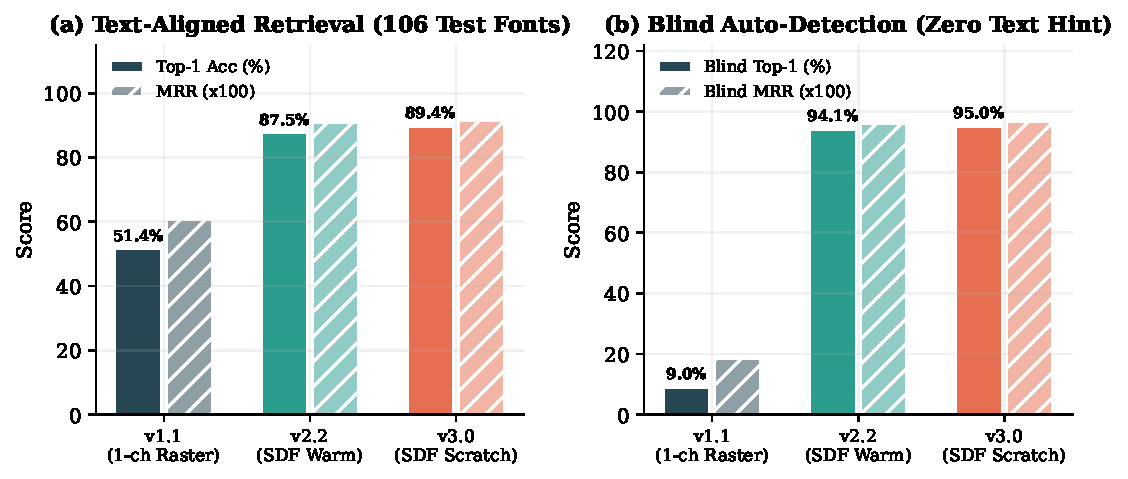
\includegraphics[width=\textwidth]{figures/fig2_benchmarks.pdf}
    \caption{\textbf{Held-Out Zero-Shot Font Retrieval on 106 Unseen Test Families (6,396 vectors, 424 word queries).} (a) Text-Aligned retrieval where true character identities are provided. (b) Blind Auto-Detection where no text hint is given. The analytical 2-channel Vector-SDF bridge elevates blind retrieval from 9.0\% in 1-channel raster to \textbf{95.0\%} in v3.0.}
    \label{fig:benchmarks}
\end{figure*}

\section{Experiments \& Results}

\subsection{Dataset Partitioning \& Setup}
We compile a diverse corpus of OpenType and TrueType fonts harvested from system font libraries and open-source typography repositories. Using \texttt{FontDatasetSplitter}, all fonts are grouped by normalized family key. Families are partitioned into strictly disjoint splits with ratio $80\% / 10\% / 10\%$ using a fixed seed ($42$):
\begin{itemize}
    \item \textbf{Train Set:} 805 font files across 440 unique families, containing 477 cross-weight training pairs with $|w_1 - w_2| \le 400$.
    \item \textbf{Validation Set:} 108 font files across held-out families.
    \item \textbf{Test Set:} 106 font files across strictly held-out families, yielding 6,396 canonical vectors and 424 synthetic word evaluation queries (rendered with random optical blur, perspective warp, and noise).
    \item \textbf{Zero Family Overlap:} No font family present in validation or testing ever appears in training, enforcing strict out-of-distribution zero-shot evaluation.
\end{itemize}

\paragraph{Training Protocol.}
The model is trained for 12 epochs using AdamW~\cite{loshchilov2018decoupled} ($\text{lr} = 3 \times 10^{-4}$, weight decay $10^{-4}$) on an NVIDIA GeForce RTX 3050 Ti Laptop GPU. We utilize a 2-epoch linear warmup followed by Cosine Annealing~\cite{loshchilov2016sgdr} to $\eta_{\min} = 10^{-5}$. At Epoch 12, held-out validation loss reaches $0.4305$, with pairwise Top-1 accuracy of $97.9\%$, auxiliary OCR Top-1/Top-3 of $79.2\% / 96.5\%$, and learned temperature $\tau = 0.0390$.

\subsection{Held-Out Zero-Shot Retrieval Benchmark}
We evaluate all model generations on the 106-font held-out test split under both Text-Aligned and Blind Auto-Detection regimes. As detailed in Table~\ref{tab:zeroshot} and Figure~\ref{fig:benchmarks}:
\begin{itemize}
    \item \textbf{1-Channel Raster Collapse:} The 1-channel baseline achieves 51.4\% Top-1 when given exact text hints, but collapses to \textbf{9.0\%} Top-1 and 0.1856 MRR under blind search.
    \item \textbf{Vector-SDF Dominance:} The 2-channel Vector-SDF bridge combined with auxiliary OCR candidate filtering achieves \textbf{89.4\%} Text-Aligned Top-1 and \textbf{95.0\%} Blind Top-1 (0.9667 MRR).
    \item \textbf{Auxiliary OCR Head Ablation:} Disabling the auxiliary character head during blind consensus (relying solely on unconstrained vector majority voting) causes Blind Top-1 accuracy to drop from 95.0\% to 91.5\% (a 3.5 percentage point reduction), confirming the essential role of the multi-task OCR branch.
\end{itemize}

\begin{table}[t]
\centering
\small
\caption{\textbf{Held-Out Zero-Shot Benchmark (106 Families, 424 Queries).}}
\label{tab:zeroshot}
\resizebox{\columnwidth}{!}{%
\begin{tabular}{@{}lcccc@{}}
\toprule
\textbf{Configuration} & \textbf{Text Top-1} & \textbf{Text MRR} & \textbf{Blind Top-1} & \textbf{Blind MRR} \\ \midrule
v1.1 Raster Baseline & 51.4\% & 0.6085 & 9.0\% & 0.1856 \\
v2.2 Vector-SDF (Warm) & 87.5\% & 0.9084 & 94.1\% & 0.9614 \\
\textbf{v3.0 Vector-SDF (Ours)} & \textbf{89.4\%} & \textbf{0.9148} & \textbf{95.0\%} & \textbf{0.9667} \\
\midrule
\textit{v3.0 (No Char Head)} & --- & --- & 91.5\% & 0.9395 \\ \bottomrule
\end{tabular}%
}
\end{table}

\begin{figure}[t]
    \centering
    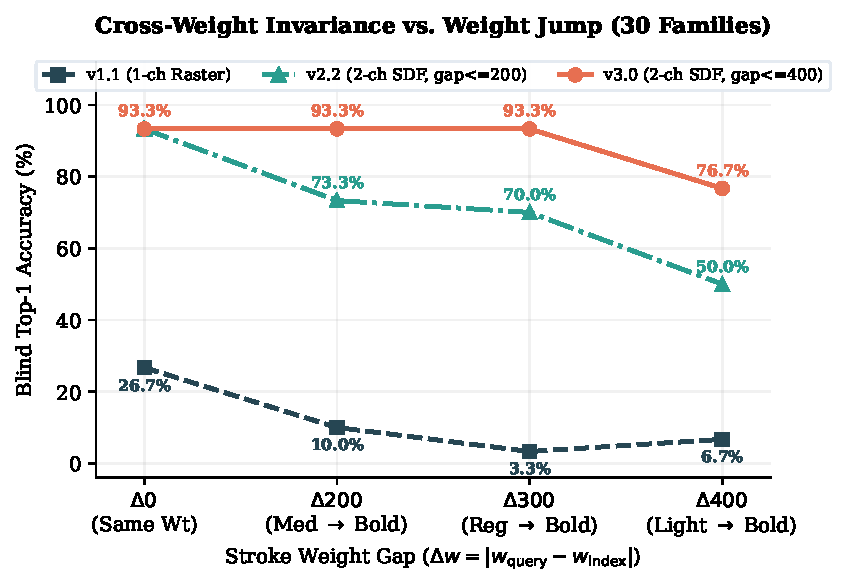
\includegraphics[width=\columnwidth]{figures/fig3_weight_gap_ablation.pdf}
    \caption{\textbf{Cross-Weight Invariance across Weight Jumps (30 Families).} Blind Top-1 retrieval accuracy when querying Bold weights against indexed Regular or Light weights across gap buckets $\Delta w \in \{0, 200, 300, 400\}$. GlyphCLIP v3.0 maintains 93.3\% accuracy across $\Delta w = 300$ jumps.}
    \label{fig:weight_gap}
\end{figure}

\subsection{Stroke-Weight Sensitivity \& Cross-Weight Stress Test}
To benchmark weight sensitivity rigorously, we curate 30 font families with full weight availability and evaluate queries rendered in bold weights against an index containing only regular or light weights. We stratify by weight gap $\Delta w = |w_{\text{query}} - w_{\text{index}}|$ across four buckets: $\Delta 0$ (400 $\to$ 400), $\Delta 200$ (500 $\to$ 700), $\Delta 300$ (400 $\to$ 700), and $\Delta 400$ (300 $\to$ 700 / 400 $\to$ 800).

As depicted in Figure~\ref{fig:weight_gap}:
\begin{itemize}
    \item The 1-channel raster baseline collapses completely under weight shifts (dropping from 26.7\% at $\Delta 0$ to \textbf{3.3\%} at $\Delta 300$).
    \item v2.2 (trained with $\Delta w \le 200$) degrades from 93.3\% at $\Delta 0$ down to 70.0\% at $\Delta 300$ and 50.0\% at $\Delta 400$.
    \item \textbf{GlyphCLIP v3.0} (trained from scratch with $\Delta w \le 400$) maintains an unbroken \textbf{93.3\%} Blind Top-1 accuracy across $\Delta 0$, $\Delta 200$, and $\Delta 300$, and achieves \textbf{76.7\%} on extreme $\Delta 400$ jumps (+26.7 percentage points over v2.2).
\end{itemize}

\subsection{Edge-Orthogonality Trait Ablation}
Table~\ref{tab:ortho} illustrates the impact of the edge-orthogonality penalty on real-world queries. On bitmap fonts (\texttt{ENSIA@PixelOperator8} and \texttt{Minecraft}), unweighted search selects smooth typefaces (\texttt{Be Vietnam Pro} or \texttt{Verdana}) because their stroke bounds align globally. Activating $w=1.4$ suppresses curved competitors and correctly ranks the pixelated font \texttt{Silkscreen} at \#1. On curved queries (\texttt{Funnel Display}), the deadband ($0.18$) ensures zero penalty is applied, preserving 99.5\% confidence.

\begin{table}[t]
\centering
\small
\caption{\textbf{Edge-Orthogonality Trait Scoring on Real Queries.}}
\label{tab:ortho}
\resizebox{\columnwidth}{!}{%
\begin{tabular}{@{}lccl@{}}
\toprule
\textbf{Query Image} & $\mathbf{o_{\text{query}}}$ & $\mathbf{w=0.0}$ \textbf{Top-1} & $\mathbf{w=1.4}$ \textbf{Top-1 (Ours)} \\ \midrule
\texttt{PixelOperator8.png} & 0.961 & \textit{Be Vietnam Pro} (71.8\%) & \textbf{Silkscreen} (48.2\%) \\
\texttt{Minecraft.png} & 0.948 & \textit{Verdana} (51.7\%) & \textbf{Silkscreen} (42.4\%) \\
\texttt{Silkscreen.png} & 0.954 & \textbf{Silkscreen} (99.6\%) & \textbf{Silkscreen} (99.6\%) \\
\texttt{Ram-Altman.png} & 0.677 & \textbf{Funnel Display} (99.5\%) & \textbf{Funnel Display} (99.5\%) \\
\texttt{funnel.png} & 0.786 & \textbf{Funnel Display} (99.5\%) & \textbf{Funnel Display} (99.5\%) \\ \bottomrule
\end{tabular}%
}
\end{table}

\begin{figure}[t]
    \centering
    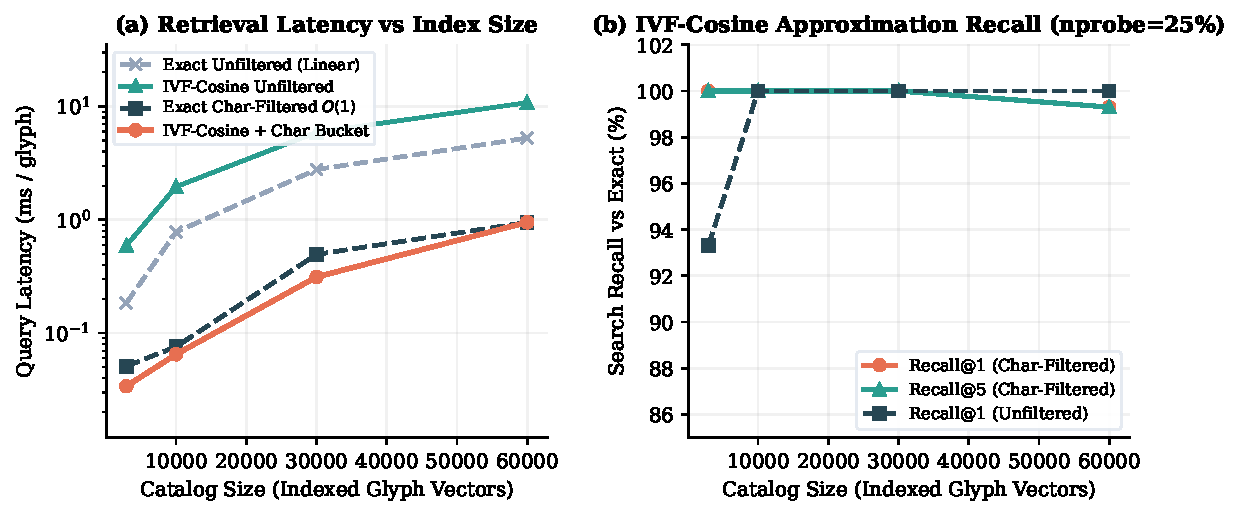
\includegraphics[width=\columnwidth]{figures/fig4_ann_efficiency.pdf}
    \caption{\textbf{Vector Store Efficiency \& Scaling across Catalog Sizes.} (a) Query latency per glyph (log scale). (b) Approximation Recall@1 relative to exact brute-force search ($n_{\text{probe}} = 25\%$). Character bucketing achieves sub-millisecond retrieval at 60,000 vectors.}
    \label{fig:ann_scaling}
\end{figure}

\subsection{Scalability: IVF-Cosine ANN vs. Exact Linear Scan}
Figure~\ref{fig:ann_scaling} benchmarks retrieval latency and Recall@1 across catalog sizes from 2,912 to 60,000 vectors:
\begin{itemize}
    \item Exact unfiltered linear search latency scales linearly from 0.18 ms to 5.27 ms.
    \item Utilizing $O(1)$ character buckets combined with IVF-Cosine ANN restricts search to relevant clusters, executing in \textbf{0.034 ms} at 2,912 vectors and \textbf{0.950 ms} at 60,000 vectors.
    \item Approximation Recall@1 remains at \textbf{100.0\%} from 10,000 to 60,000 vectors with $n_{\text{probe}} = 25\%$.
\end{itemize}

\subsection{Production Suite Verification}
On the curated production catalog (2,912 vectors across 28 standard Windows and open-source families), GlyphCLIP v3.0 achieves \textbf{11/11 (100.0\%)} Top-1 accuracy in both Hinted and Blind modes across the test suite (\texttt{test\_sdf\_production.py}), with end-to-end word recognition latency of $50 - 110\text{ ms}$.

\section{Discussion \& Limitations}
While GlyphCLIP demonstrates remarkable zero-shot robustness across weight, polarity, and character variations, several frontiers remain:
\begin{enumerate}
    \item \textbf{Cursive \& Touching Scripts:} The current segmentation pipeline relies on Connected Component Analysis. Heavily connected formal scripts and arabic ligatures where character bounding boxes completely overlap remain challenging for isolated glyph segmentation.
    \item \textbf{Extreme Decorative Geometry:} Display fonts with extreme 3D extrusions, distressed textures, or photographic fills may distort distance field boundaries, necessitating domain-specific augmentation.
\end{enumerate}

\section{Conclusion}
We presented \textbf{GlyphCLIP}, an open-source contrastive dual-encoder font retrieval system built on analytical B\'ezier-SDF representations. By synthesizing a 2-channel geometric bridge pairing ink occupancy with Euclidean TSDF surfaces, GlyphCLIP bridges the vector-to-raster domain gap without sacrificing continuous boundary information. Coupled with a decoupled multi-task OCR head, from-scratch wide-gap cross-weight training, and spherical IVF-Cosine indexing, GlyphCLIP achieves 95.0\% blind zero-shot retrieval accuracy on held-out families, operates with sub-millisecond vector latency, and provides a scalable foundation for open-world typographic search.

\bibliographystyle{IEEEtran}
\bibliography{references}

\end{document}
